	%%%Architettura alto livello%%%
\section{Architettura ad alto livello}
Nella seguente sezione verr\`{a} illustrata l'architettura ad alto livello del sistema sviluppato, 
escludendo i dettagli implementativi e legati al linguaggio. Viene fornito un diagramma delle componenti per mostrare
molto ad alto livello l'architettura del sistema.\\
\begin{center}
\begin{figure}[h!]
	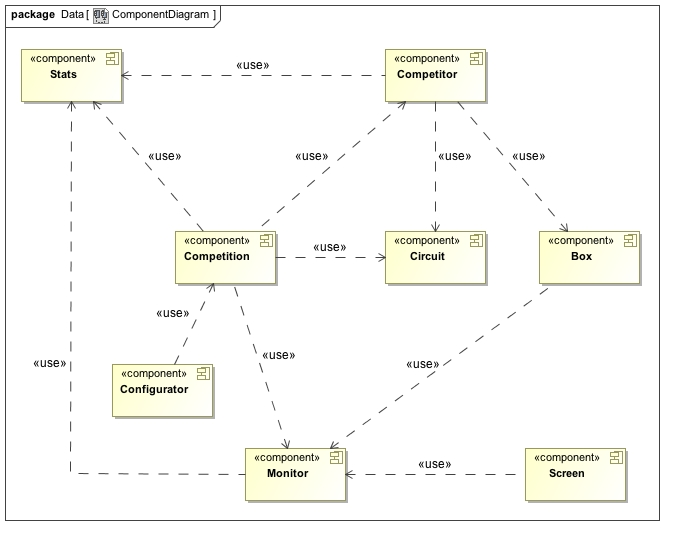
\includegraphics[scale=0.50]{img/ComponentDiagram.jpg}
	\caption{Diagramma delle componenti}
\end{figure}
\end{center}
% Componenti del sistema
\subsection{Componenti di sistema}
Le principali componenti del sistema sono:
\subsubsection{Competition}
La \emph{Competition} \`{e} l'unit\`{a} atta ad orchestrare l'avvio e la conclusione della corsa. Tale componente, dunque, \`{e} stata concepita per 
offrire le seguenti funzionalit\`{a}:
\begin{itemize}
\item Configurazione parametri di gara:
	\begin{itemize}
		\item numero di giri;
		\item numero di concorrenti;
		\item circuito;
	\end{itemize}
\item Gestione della sessione di iscrizione e accettazione concorrenti (configurati a livello della componente \emph{Box})
\item Avvio delle componenti necessarie al monitoraggio della gara (quali ad esempio \emph{Monitor})
\item Avvio controllato della competizione vera e propria nel momento in cui tutti i prerequisiti di inizio sono soddisfatti, ovvero:
\begin{itemize}
\item la competizione \`{e} stata configurata correttamente;
\item le componenti di controllo e gestione della competizione sono attive e in attesa di comandi;
\item i concorrenti sono stati correttamente registrati alla competizione e in attesa di partire;
\end{itemize}
\end{itemize}
\subsubsection{Competitor}
Il \emph{Competitor} \`{e} l'entit\`{a} pensata ad svolgere la gara. \`{E} caratterizzato dalle seguenti sotto-componenti:
\begin{itemize}
\item \textbf{Auto}, ovvero tutte le caratteristiche fisiche legate all'auto, ovvero:
	\begin{itemize}
		\item motore;
		\item capacit\`{a} del serbatoio;
		\item massima accelerazione;
		\item massima velocit\`{a};
		\item gomme montate (mescola, modello, tipo);
		\item livello usura gomme;
		\item livello della benzina nel serbatoio;
	\end{itemize}
\item \textbf{Guidatore}, cio\`{e} le informazioni che descrivono pi\`{u} dettagliatamente il concorrente in gara:
	\begin{itemize}
		\item nome e cognome pilota;
		\item nome scuderia
	\end{itemize}
\item \textbf{Strategia}, ovvero la strategia che sta adottando il pilota, suggerita dai box e dinamica nel corso della gara:
	\begin{itemize}
		\item stile di guida, variabile tra conservativo, normale, aggressivo, a seconda dello stato della macchina e delle
			previsioni fatte dai box
		\item numero di lap prima del pit stop
		\item addizionalmente, quando viene fatto un pit stop, la strategia determina anche quali siano le nuove gomme da montare,
		 	la quantit\`{a} di benzina da avere nel serbatoio e il tempo impiegato per il pit stop.
	\end{itemize}
\end{itemize}
Tutte queste informazioni insieme creano quello che viene definito il concorrente di gara. 
Tali informazioni verranno poi usate nel corso della gara per:
	\begin{itemize}
		\item scegliere al momento giusto la miglior traiettoria da seguire, in base alla presenza o meno di altri concorrenti
			nelle vicinanze e alla difficolt\`{a} del tratto;
		\item fornire costantemente aggiornamenti sul suo stato (tramite una parte del modulo \emph{Stats}, informando il computer di bordo
			riguardo a:
			\begin{itemize}
				\item livello di usura gomme;
				\item livello di benzina;
				\item checkpoint attraversato con tempo di arrivo;
				\item insieme al checkpoint verranno aggiornate le informazioni relative a settore e lap;
				\item velocit\`{a} massima raggiunta.
			\end{itemize}
		\item contattare ad ogni giro il box per ottenere una strategia aggiornata;
		\item se suggerito dai box, effettuare un pitstop;
		\item ritirarsi dalla gara una volta che le condizione dell'auto non permettano di poter correre ulteriormente;
		\item banalmente, continuare a correre fino alla fine delle lap prestabilite, dopodich\`{e} fermarsi.
	\end{itemize}
\subsubsection{Circuit}
Il circuito \`{e} una risorsa finalizzata ad offrire il piano su cui svolgere la competizione. \`{E} condivisa fra tutti i concorrenti in gara e
offre un insieme di funzionalit\`{a} per poter conoscere le caratteristiche dei vari tratti della pista (compresi i concorrenti presenti
al momento dell'attraversamento). \`{E} composto dalle seguenti sottocomponenti:
\begin{itemize}
\item \textbf{Checkpoint}:
i \emph{Checkpoint} rappresentano punti di arrivo intermedi del circuito. Come una suddivisione in fette da 1 secondo possono discretizzare 1 minuto,
cos\`{i} i \emph{Checkpoint} discretizzano il circuito. Ogni \emph{Checkpoint} introduce un tratto della pista potenzialmente diverso da quello precedente.
Per esempio, il $\emph{Checkpoint}_n$ potrebbe essere il punto di entrata di un tratto della pista accessibile ad un numero massimo di 4 concorrenti insieme,
mentre il successivo $\emph{Checkpoint}_{n+1}$ potrebbe esporre un tratto pi`{u} stretto e quindi accessibile solo a 2 concorrenti. Schematizzando, 
il \emph{Checkpoint} \`{e} caratterizzato da:
\begin{itemize}
\item \textbf{molteplicit\`{a}}: ovvero il numero di concorrenti che possono trovarsi contemporaneamente nel tratto a seguire;
\item \textbf{posizione nella pista}: un \emph{Checkpoint} pu\`{u} essere il traguardo, l'inizio del settore, la fine di un settore, all'uscita dei box, l'entrata
					per i box, i box oppure un punto intermedio fra altri due \emph{Checkpoint};
\item \textbf{tempi di arrivo}: ogni \emph{Checkpoint} tiene traccia dell'istante in cui un concorrente ci \`{e} passato sopra.
\end{itemize}
\item \textbf{Path}: rappresenta una delle possibili traiettorie da usare per andare da un \emph{Checkpoint} a quello successivo. La traiettoria presenta
	un numero di \emph{Path} uguale alla molteplicit\`{a} del \emph{Checkpoint} che la precede. Ogni \emph{Path} \`{e} descritto da:
	\begin{itemize}
		\item lunghezza
		\item angolo
		\item grip, ovvero l'aderenza sul tratto
	\end{itemize}
Normalmente i path appartenenti allo stesso tratto differiscono di poco.
\item \textbf{Iteratore}: l'unit\`{a} permette di sapere la struttura della pista. Si suppone venga usata per sapere quale \emph{Checkpoint} ne segue un altro,
	oppure per sapere dove sia il \emph{Checkpoint} di inizio box. 
\end{itemize}
\subsubsection{Stats}
Questa componente mantiene la storia della gara e offre un insieme di funzionalit\`{a} che permettono di elaborare tali dati per offrirne differenti viste:
	\begin{itemize}
		\item migliori performance in un determinato istante di tempo
		\item classifica aggiornata per istante di tempo
		\item informazioni sui concorrenti relative ad un particolare lap, checkpoint o settore (in una specifica lap);
	\end{itemize}
\subsubsection{Box}
Il \emph{Box} \`{e} l'entit\`{a} che si occupa di gestire la configurazione e la corsa di un concorrente. Durante la competizione, il \emph{Box} verifica costantemente
lo stato dell'auto e fornisce eventuali cambi di strategia se ritenuto opportuno. Inoltre decide quando i pitstop del concorrente con tutte le caratteristiche 
ad esso legate, quali:
	\begin{itemize}
		\item benzina da aggiungere nel serbatoio
		\item gomme da montare
	\end{itemize}
Ogni \emph{Box} \`{e} caratterizzato da uno fra 4 tipi di strategia, diversi per grado di ``ottimismo'' nelle valutazioni e nei calcoli dati lo stato della 
macchina, le medie calcolate e lo stile di guida del concorrente:
	\begin{enumerate}
		\item \textbf{Cautious}: cauto, sottostima il numero di giri ancora fattibili;
		\item \textbf{Normal}: stima abbastanza realistica delle possibilit\`{a} del concorrente, considera anche un margine di errore nei calcoli
			per effettuare una valutazione;
		\item \textbf{Risky}: le stime vengono effettuate in base a calcoli esatti che di solito non tengono in considerazione fattori che nella
			realt\`{a} possono incidere in modo negativo;
		\item \textbf{Fool}: nella realt\`{a} normalmente non si arriva a tanto, ma per fini di test \`{e} stato inserito anche un tipo di strategia
			che sovrastima le possibilit\`{a} del concorrente, portandolo a squalifica quasi certa.
	\end{enumerate}
Ci\`{o} che il box suggerisce al concorrente durante la gara \`{e}:
	\begin{itemize}
		\item stile di guida. Verr\`{a} suggerito uno stile pi\`{u} conservativo se i consumi si sono rivelati maggiori del previsto e viceversa;
		\item numero di lap al pitstop
	\end{itemize}
Il \emph{Box} riceve informazioni sullo stato del concorrente alla fine di ogni settore e ricalcola la strategia alla fine del secondo settore. Il concorrente
richiede la nuova strategia al box in prossimit\`{a} del checkpoint dove \`{e} possibile proguire o andare ai box.\\
\`{E} sembrato pi\`{u} realistica la scelta di non calcolare la strategia alla fine del terzo settore, perch\`{e} si suppone che nella realt\`{a} non si possa essere
cos\`{i} veloci da calcolare una nuova strategia istantaneamente alla fine del circuito con i dati del terzo settore. \`{E} piuttosto pi\`{u} probabile che 
qualunque cambio di strategia o richiesta di rientro ai box venga stabilita gi\`{a} alla fine del secondo settore. In modo che in prossimit\`{a} dei box il concorrente
possa ottenere l'informazione istantaneamente e possa quindi decidere come e dove procedere.
\subsubsection{Monitor}
La componente \emph{Monitor} e costituita dall'insieme delle unit\`{a} concepite per esporre le informazioni e i dati prodotti a basso livello
dal simulatore. Ne esistono due tipi:
\begin{itemize}
	\item \textbf{monitor di competizione}: utilizzato per offrire informazioni riguardanti la gara e i singoli concorrenti;
	\item \textbf{monitor di box}: utilizzato per esporre i dati relativi alle computazioni del box, e le informazioni grezze legate al
		concorrente appartenente alla sua scuderia e i dati rielaborati di settore in settore per formulare nuove strategie.
\end{itemize}
\subsubsection{Screen} 
Gli \emph{Screen} sono la parte pi\`{u} alta del sistema. Servono a mettere in connessione l'utente finale e la parte logica del simulatore.
Tramite gli \emph{Screen} \`{e} possibile ricevere aggiornamenti grafici (di base) sullo stato di avanzamento della simulazione sotto il punto di vista 
dei singoli box o della gara complessiva.
\subsubsection{Configurator}
Questa componente offre la possibilit\`{a} di configurare le parti parametriche del sistema, ovvero:
\begin{itemize}
	\item concorrenti 
	\item competizione (i parametri elencati nella sezione \emph{Competition}
	\item box
\end{itemize}
Il \emph{Configurator} ha inoltre l'onere di inviare i parametri cos\`{i} configurati alle componenti opportune.

 \subsubsection{Radio}
La componente radio \`{e} stata creata per gestire la comunicazione remota fra le componenti distribuite.\\
Il sistema inizialmente \`{e} stato implementato con supporto solo all'esecuzione locale. Si conoscevano le componenti che sarebbero state distribuite,
ma il processo di separazione \`{e} avvenuto successivamente. Quindi per agevolare tale processo si \`{e} pensato di demandare l'onere della comunicazione 
tra queste componenti a unit\`{a} specializzate, chiamate appunto radio. In questo modo \`{e} stato pi\`{u} soft il passaggio da locale a distribuito,
che ha richiesto di rivedere solo le componenti \emph{Radio}.\\\\
\emph{\textsc{Nota Bene}}:\\
La componente \emph{Radio} costituisce un layer di supporto alla comunicazione 
distribuita delle componenti. Considerando che a questo livello del documento non \`{e} ancora il momento di scendere nei dettagli fino a discutere 
della distribuzione, si pensa sia sufficiente averla nominata nella descrizione delle componenti. Verr\`{a} ripresa
in considerazione successivamente nel documento. Inserendola ora nei diagrammi delle componenti rischierebbe di confondere la visione di insieme
del sistema.
% Interazione fra le componenti
\subsection{Interazione fra le componenti}
Nella seguente sezione verranno spiegate le interazione principali fra le componenti.\\\\
\subsubsection{Configurator-Competition}
\begin{center}
\begin{figure}[h!]
	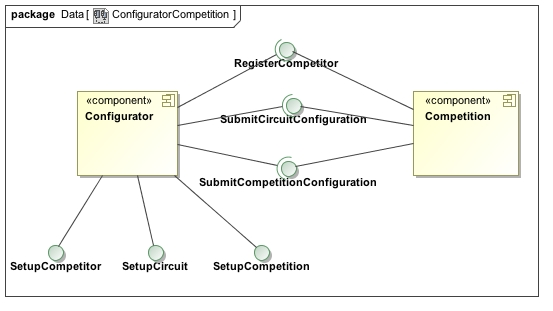
\includegraphics[scale=0.55]{img/InteractionDiagram/Implementation_Diagram__ConfiguratorCompetition.jpg}
\caption{Interface component diagram - Configurator/Competition}
\end{figure}
\end{center}
Al livello pi\`{u} alto della fase di configurazione c'\`{e} la componente \emph{Configurator}, la quale viene utilizzata per impostare i parametri
relativi alla \emph{Competition}. Tali parametri vengono prima impostati dall'utente (o letti da file) tramite le interfacce \textbf{SetupCompetitor},
\textbf{SetupCompetition} e \textbf{SetupCircuit} e successivamente inviati alla componente \emph{Competition} per l'inizializzazione.\\
\textbf{RegisterCompetitor} \`{e} utilizzata una volta per ogni competitor da iscrivere.
\subsubsection{Competition-Competitor}
\begin{center}
\begin{figure}[h!]
	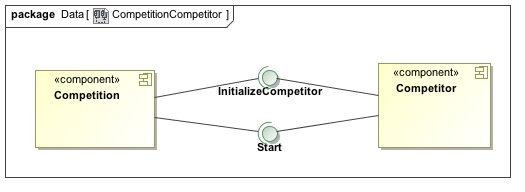
\includegraphics[scale=0.55]{img/InteractionDiagram/Implementation_Diagram__CompetitionCompetitor.jpg}
\caption{Interface component diagram - Competition/Competitor}
\end{figure}
\end{center}
L'interazione fra la \emph{Competition} e il \emph{Competitor} avviene, come per le altre interazioni \emph{Competition}-componente in fase di configurazione
e avvio. La \emph{Competition} si occupa di ricevere i parametri relativi a ogni \emph{Competitor} dal \emph{Configurator} (come verr\`{a} spiegato fra poco) per 
poi inizalizzare il competitor. Quando tutti i concorrenti sono pronti e anche i \emph{Box}, l'interfaccia \textbf{Start} verr\`{a} utilizzata per dare il
via ai concorrenti.
\subsubsection{Competition-Monitor}
\begin{center}
\begin{figure}[h!]
	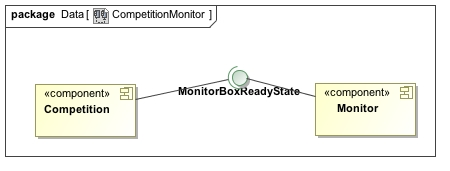
\includegraphics[scale=0.55]{img/InteractionDiagram/Implementation_Diagram__CompetitionMonitor.jpg}
\caption{Interface component diagram - Competition/Monitor}
\end{figure}
\end{center}
L'interazione \emph{Competition}-\emph{Monitor} riguarda solo una piccola fase dell'inizializzazione, processo che verr\`{a} esplicato in dettaglio in seguito.
A concorrenti registrati, la \emph{Competition} sfruttera un interfaccia offerta dal monitor per sapere quando tutti i \emph{Box} sono pronti e avviati.
L'interfaccia \`{e} l'unica illustrata in figura.
\subsubsection{Competition-Circuit}
\begin{center}
\begin{figure}[h!]
	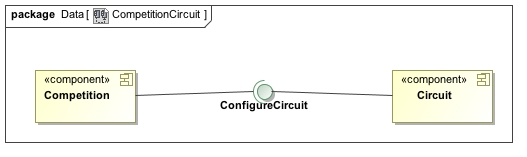
\includegraphics[scale=0.55]{img/InteractionDiagram/Implementation_Diagram__CompetitionCircuit.jpg}
\caption{Interface component diagram - Competition/Circuit}
\end{figure}
\end{center}
Anche in questo caso, l'interazione \emph{Competition}-\emph{Circuit} si ha in fase di inizializzazione quando le due componenti entrano in contatto
per la configurazione. La \emph{Competition} inizializza cio\`{e} il circuito impostando i parametri che lo caratterizzano, quali:
	\begin{itemize}
		\item numero di checkpoint
		\item caratteristiche dei tratti fra checkpoint (lunghezza, angolo ...)
		\item posizione dei checkpoint di entrata e uscita box
		\item posizione del checkpoint traguardo
	\end{itemize}
\subsubsection{Competition-Stats}
\begin{center}
\begin{figure}[h!]
	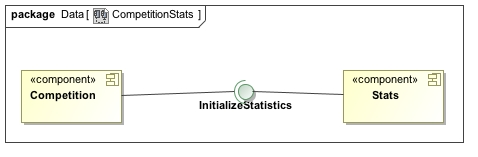
\includegraphics[scale=0.55]{img/InteractionDiagram/Implementation_Diagram__CompetitionStats.jpg}
\caption{Interface component diagram - Competition/Stats}
\end{figure}
\end{center}
La componente \emph{Stats} ottiene i parametri di configurazione in fase di inizalizzazione dalla \emph{Competition}, tramite
\textbf{InitilizeStatistics}.
\subsubsection{Competitor-Stats}
\begin{center}
\begin{figure}[h!]
	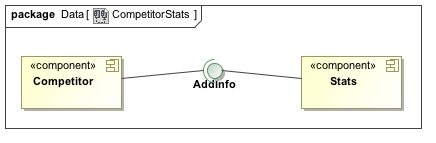
\includegraphics[scale=0.55]{img/InteractionDiagram/Implementation_Diagram__CompetitorStats.jpg}
\caption{Interface component diagram - Competitor/Stats}
\end{figure}
\end{center}
La componente \emph{Stats} offre al \emph{Competitor} l'interfaccia \textbf{AddInfo} che il concorrente utilizza per fornire costantemente a \emph{Stats}
dati aggiornati riguardo alla gara in corso (dati relativi al singolo concorrente). Ad ogni checkpoint quindi il concorrente manda un aggiornamento
a \emph{Stats} che poi verranno utilizzate per effettuare calcoli di insieme riguardo alla gara o per essere mandate a chi le richiedesse.
\subsubsection{Competitor-Circuit}
\begin{center}
\begin{figure}[h!]
	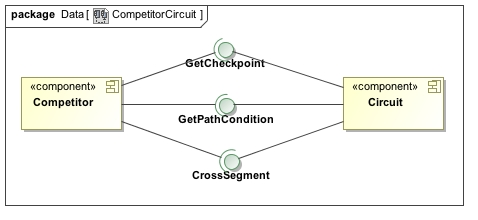
\includegraphics[scale=0.55]{img/InteractionDiagram/Implementation_Diagram__CompetitorCircuit.jpg}
\caption{Interface component diagram - Competitor/Circuit}
\end{figure}
\end{center}
L'interazione \emph{Competitor}-\emph{Circuit} avviene durante lo svolgimento della competizione. Il concorrente sfrutta le interfacce del \emph{Circuit}
per ottenere informazioni sul circuito e ``informarlo'' degli spostamenti nel corso della gara.\\
\textbf{GetCheckpoint} garantisce che il concorrente ottenga sempre il checkpoint corretto a seconda della posizione corrente.
\textbf{GetPathCondition} permette di ottenere informazioni sulle caratteristiche statiche e dinamiche della tratto da attraversare. Le caratteristiche 
dinamiche sono legate ai concorrenti attualmente presenti sul tratto.
\textbf{CrossSegment} assicura che il tratto possa essere attraversato senza collisioni e che il \emph{Circuit} possa tracciare l'avvenuto passaggio 
dell'auto.
\subsubsection{Monitor-Stats}
\begin{center}
\begin{figure}[h!]
	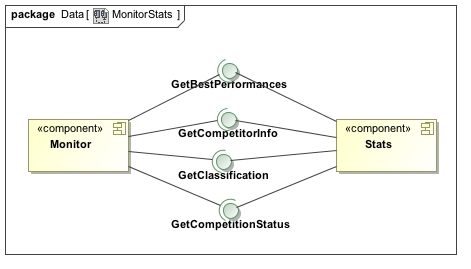
\includegraphics[scale=0.55]{img/InteractionDiagram/Implementation_Diagram__MonitorStats.jpg}
\caption{Interface component diagram - Monitor/Stats}
\end{figure}
\end{center}
La componente \emph{Monitor} si appoggia a \emph{Stats} per poter reperire le informazioni da essere esposte. Per questo motivo
\emph{Stats} offre un insieme di interfacce finalizzate a fornire i dati grezzi di competizione sotto forma di viste utili alla ``pubblicazione''.\\
\textbf{GetBestPerformance} fornisce i migliori tempi relativi a settori e giro.\\
\textbf{GetCompetitorInfo} reperisce informazioni legate al singolo concorrente, come ad esempio lo stato della macchina ad un determinato istante.\\
\textbf{GetClassification}, come dice il nome, ritorna informazioni legate alla classifica.\\
\textbf{GetCompetitionStatus} espone informazioni legate alla competizione nel suo insieme, come ad esempio la posizione dei concorrenti nel circuio
in un determinato istante di tempo.
\subsubsection{Configurator-Box}
\begin{center}
\begin{figure}[h!]
	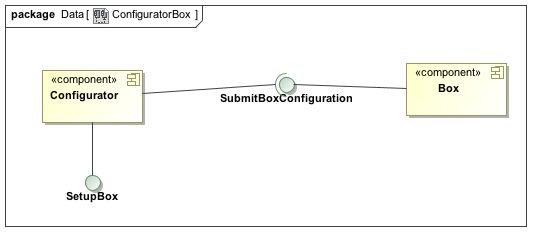
\includegraphics[scale=0.55]{img/InteractionDiagram/Implementation_Diagram__ConfiguratorBox.jpg}
\caption{Interface component diagram - Configurator/Box}
\end{figure}
\end{center}
La componente \emph{Configurator} offre anche la possibilit\`{a} di configurare un \emph{Box}. Per questo motivo il \emph{Box} espone un'interfaccia
da utilizzare per sottomettere i parametri di configurazione. 
\subsubsection{Box-Monitor}
\begin{center}
\begin{figure}[h!]
	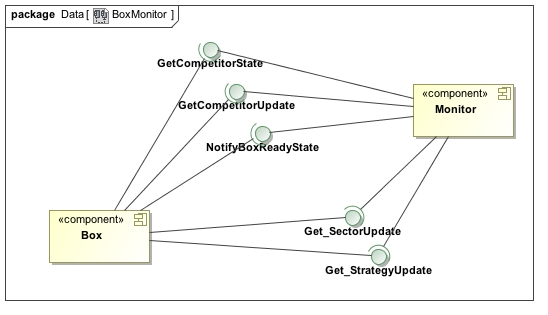
\includegraphics[scale=0.55]{img/InteractionDiagram/Implementation_Diagram__BoxMonitor.jpg}
\caption{Interface component diagram - Box/Monitor}
\end{figure}
\end{center}
La prima interazione che la componente \emph{Box} ha con il \emph{Monitor} \`{e} in fase di inizializzazione della gara. La sequenza di azioni verr\`{a} esplicata
dettagliatamente in seguito, per ora basti sapere che il \emph{Box}, una volta configurato e pronto per monitorare la gara ed elaborare i dati del suo
concorrente, dovr\`{a} mandare una notifica tramine la componente \emph{Monitor} utilizzando \textbf{NotifyBoxReadyState}.\\
Le rimanenti due interfacce sono utilizzate per reperire informazioni sullo stato del concorrente (livello di benzina rimasta, usura gomme...) e
aggiornamenti riguardo al posizionamento e tempi del concorrente durante la gara.
\subsubsection{Screen-Monitor}
\begin{center}
\begin{figure}[h!]
	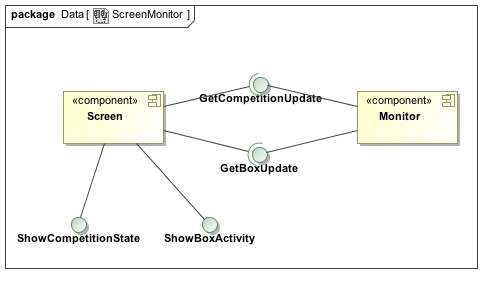
\includegraphics[scale=0.55]{img/InteractionDiagram/Implementation_Diagram__ScreenMonitor.jpg}
\caption{Interface component diagram - Screen/Monitor}
\end{figure}
\end{center}
La componente \emph{Screen} comunica con il \emph{Monitor} per ottenere informazioni utili da esporre graficamente all'utente. Tali
informazioni possono riguardare la competizione in senso globale, oppure essere legate ai singoli concorrenti e box.
\subsubsection{Competitor-Box}
\begin{center}
\begin{figure}[h!]
	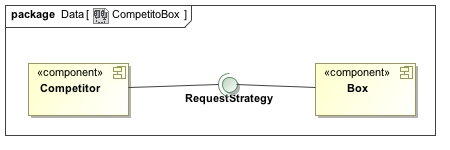
\includegraphics[scale=0.55]{img/InteractionDiagram/Implementation_Diagram__CompetitoBox.jpg}
\caption{Interface component diagram - Competitor/Box}
\end{figure}
\end{center}
Man mano che la competizione procede, il \emph{Box} colleziona i dati di gara del rispettivo concorrente per calcolarne medie e statistiche. 
A partire da queste informazioni produce una nuova strategia ogni giro. Per questo offre un'interfaccia \textbf{RequestStrategy} che il concorrente
utilizza nel corso della gara per ottenere suggerimenti utili per proseguire. La strategia fornita dal \emph{Box} potrebbe anche richiedere 
un pitstop per un rifornimento benzina e cambio gomme.
% Strategia adottata per la correttezza temporale
\subsubsection{Strategia di simulazione}
In questa sezione viene spiegata la strategia che è stata adottata per ottenere una simulazione realistica della gara. Le problematiche da 
affrontare sono già state discusse nel capitolo \ref{problematiche_concorrenza}.\\ 
La soluzione prevede l'esistenza di concorrenti che simultaneamente percorrono il circuito e un insieme di entità di supporto per evitare 
i problemi visti. Tali entità sono:
\begin{itemize}
  \item \textbf{coda al checkpoint}: ogni checkpoint introduce tratti di circuito con caratteristiche diverse rispetto a quello precedente.
	      \`{E} quindi possibile che 
  \item \textbf{istante di arrivo}:
  \item \textbf{istante limite di arrivo previsto}:
  \item \textbf{istante di liberazione traiettoria}:
\end{itemize}
% Dimostrazione dell'assenza di stallo
\subsubsection{Assenza di stallo}

%%% Architettura in dettaglio %%
\subsection{Architettura in dettaglio}
% Elenco dei task con descrizione
\subsubsection{Risorse attive}
% Elenco risorse condivise con descrizione
\subsubsection{Risorse passive}
\begin{itemize}
\item{Risorse protette}
\item{Altre risorse}
\end{itemize}
%"Analisi della concorrenza"
\subsubsection{Analisi della concorrenza}
	%. analisi dell'interazione risorse e task (senza menzionare la distribuzione)
	%. dimostrazione assenza di racecondition
	%. dimostrazione assenza di starvation
\begin{itemize}
\item{Interazione tra risorse condivise e task}
\item{Assenza di racecondition}
\item{Assenza di starvation}
\end{itemize}
%"Distribuzione"
\subsubsection{Distribuzione}
	%. Elenco risorse distribuite
	%. Interazione risorse distribuite
	%. Misure di fault tolerance
\begin{itemize}
\item{Componenti distribuite}%Con motivazione
\item{Interazione fra le componenti distribuite}
\item{Misure di fault tolerance}
\end{itemize}
% Inizializzazione gara
\subsection{Inizializzazione competizione}
% Stop gara
\subsection{Stop competizione}
